\documentclass[oneside]{ausarbeitung}
\bibliography{latexlit}


% ----------------------------------------------------------------------

\begin{document}

%--- Sprachauswahl
% Erlaubte Werte:
%   \selectlanguage{english}
%   \selectlanguage{ngerman}
\selectlanguage{ngerman}

%--- Art der Arbeit
% Erlaubte Werte:
%   \Praxissemesterbericht
%   \Projektbericht
%   \Bachelorarbeit
%   \Seminararbeit
%   \Masterarbeit

\Projektbericht

%--- Studiengang:
% Erlaubte Werte:
%   \Informatik
%   \Elektronik
%   \DataScience
\Informatik

\title{Where tf am I?}

\author{Niklas Fichtner; Hikmet Gözaydin; Oskar Pokorski}
\matrikelnr{85822; 85987; 81749}

%--- Ist der Erstbetreuer (\examinerA) an der Hochschule ein Professor?
% Erlaubte Werte:
%   \examinerIsAProfessortrue   % Ja
%   \examinerIsAProfessorfalse  % Nein
\examinerIsAProfessortrue   % Ja

%--- Betreuer
\examinerA{Stefan Wehrenberg}
%\examinerB{Prof.~Dr.~Ulrich~Klauck}

%--- Einreichungsdatum
\date{20. Juli 2025}

%--- Angaben zur Firma
% Auskommentieren, wenn die Arbeit nicht bei einer ext. Firma gemacht wurde.
%\companyname{Beispielfirma}
%\industrialsector{Beispielbranche}
%\department{Beispielabteilung}
%\companystreet{Beispielstr. 1}
%\companycity{12345 Musterstadt}

%--- Angaben zum Betreuer bei dieser Firma
%\advisorname{Name des Betreuers}
%\advisorphone{(01234) 567-890}
%\advisoremail{name@company.xxx}

%--- Titelseite Anzeigen
\maketitle
\cleardoublepage

%---
\pagenumbering{roman}
\setcounter{page}{1}

%--- Firmendaten Anzeigen
% Auskommentieren, wenn die Arbeit nicht bei einer ext. Firma gemacht wurde.
%\makeworkplace
%\cleardoublepage

%--- Sperrvermerk (Funktioniert nur bei externen Bachelor- oder Masterarbeiten.)
\makeconfidentialclause
\cleardoublepage


%-----------------------------------------------------------------------
\cleardoublepage
\tableofcontents

%---
\listoffigures

%---
\listoftables


%---


\cleardoublepage
\pagenumbering{arabic}
\setcounter{page}{1}

% ----------------------------------------------------------------------
\chapter{Einleitung}
\label{cha:einleitung}

WTFAI: Where tf am I ist ein levelbasiertes Action-Plattform-Spiel, in dem die Spieler in eine unbekannte, gefährliche Welt geworfen werden – ohne Kontext, ohne klare Hinweise, nur mit dem Ziel, das Portal am Ende jedes Levels lebend zu erreichen. Auf dem Weg dorthin müssen sie feindlichen Kreaturen ausweichen oder sie im Kampf besiegen. Gleichzeitig gilt es, stets auf die eigenen Lebenspunkte zu achten, denn ein falscher Schritt oder zu viel Schaden bedeutet das Ende des Versuchs.

Das Spiel richtet sich an Jugendliche und junge Erwachsene ab etwa 12 Jahren, die Spaß an schnellen, fordernden Spielen mit actionreichen Elementen haben.

Entwickelt wurde WTFAI mit der Unreal Engine 5. Durch den Einsatz von Fab-Assets konnten wir realistische und detailreiche Umgebungen erschaffen, die zur mysteriösen und bedrohlichen Stimmung des Spiels beitragen. Die leistungsstarken Werkzeuge von UE5 ermöglichten es uns, hochwertige visuelle Effekte und flüssige Animationen in kurzer Entwicklungszeit umzusetzen.


%---
\chapter{Gameplay und Mechaniken}
\label{cha:gameplayundmechaniken}

\section{Spielmechaniken}
\label{sec:spielmechaniken}

Da unser Speil Lebelbassiert ist, ist dies auch die Core Gameplay Loop. Somit ist die Hauptspielmechanik ins Portal am Ende vom Level zu kommen.
Dabei muss man die Gegner besieten oder ihnen ausweichen und darauf achten, dass seine Lebenspunkte nicht auf Null fallen. 


\section{Progression und Leveldesign}
\label{sec:progressionundleveldesign}

Das Spiel \textit{Where tf am I?} besteht aus fünf einzigartigen Leveln, die den Spieler schrittweise an die Spielmechaniken heranführen und zunehmend komplexere Herausforderungen bieten. Die Progression ist so gestaltet, dass der Spieler kontinuierlich seine Fähigkeiten verbessert und seine Geschicklichkeit sowie strategisches Denken weiterentwickelt. Jedes Level führt neue Elemente ein, die auf den vorherigen aufbauen, um ein motivierendes und abwechslungsreiches Spielerlebnis zu schaffen, ohne den Spieler zu überfordern.

Die Progression im Spiel basiert auf einer klaren Abfolge von Leveln, die den Spieler schrittweise an die zentralen Mechaniken – Bewegung, Sprungtechnik und Kampf – heranführt und gleichzeitig die Komplexität steigert. Anfangs liegt der Fokus auf der Einführung der grundlegenden Steuerung und Spielphysik, wobei der Schwierigkeitsgrad niedrig gehalten wird, um einen leichten Einstieg zu ermöglichen. Im Verlauf des Spiels werden neue Gegnerarten, komplexere Levelumgebungen und anspruchsvollere Jump’n’Run-Passagen eingeführt, die den Spieler dazu zwingen, seine erlernten Fähigkeiten zu kombinieren. Die Levelstruktur ist so konzipiert, dass sie eine ausgewogene Lernkurve bietet: Während frühe Level die Spielmechaniken vermitteln, fordern spätere Level strategisches Denken und präzises Timing. Die dunkle Gestaltung des finalen Levels stellt den Höhepunkt der Progression dar, indem sie alle erlernten Fähigkeiten in einer komplexen Umgebung testet, um ein herausforderndes Spielerlebnis zu schaffen.

\subsection{Level 1}
\label{sub:level1}

\textbf{Level 1} ist als Einführung in die grundlegenden Spielmechaniken konzipiert. Der Spieler lernt die Steuerung (WASD zum Bewegen, Leertaste zum Springen, Linksklick zum Schießen) durch eine kurze Anleitung kennen. Das Level ist bewusst kurz und übersichtlich gestaltet, um einen schnellen Einstieg zu ermöglichen und den Spieler mit den grundlegenden Bewegungs- und Kampfmechaniken vertraut zu machen.


\subsection{Level 2}
\label{sub:level2}


\textbf{Level 2} dient dazu, dem Spieler ein besseres Verständnis für die Bewegungs- und Sprungmechaniken zu vermitteln und ihn mit neuen Gegnertypen vertraut zu machen.
Der Ablauf beginnt mit einem Kampf gegen die robusten „Tank“-Gegner, gefolgt von einer Auseinandersetzung mit dem schnellen Schnellschuss-Magier.
Zum Abschluss absolviert der Spieler ein kurzes Jump’n’Run, an dessen Ende sich ein Portal befindet, das den Übergang zum nächsten Level ermöglicht.


\subsection{Level 3}
\label{sub:level3}

\textbf{Level 3} sieht aus wie ein Gefängnis und hat zwei Etagen. Im ersten Bereich muss man viele Gegner besiegen und ihren Angriffen ausweichen, um nach oben zu kommen.
\begin{figure}[H]
    \centering
    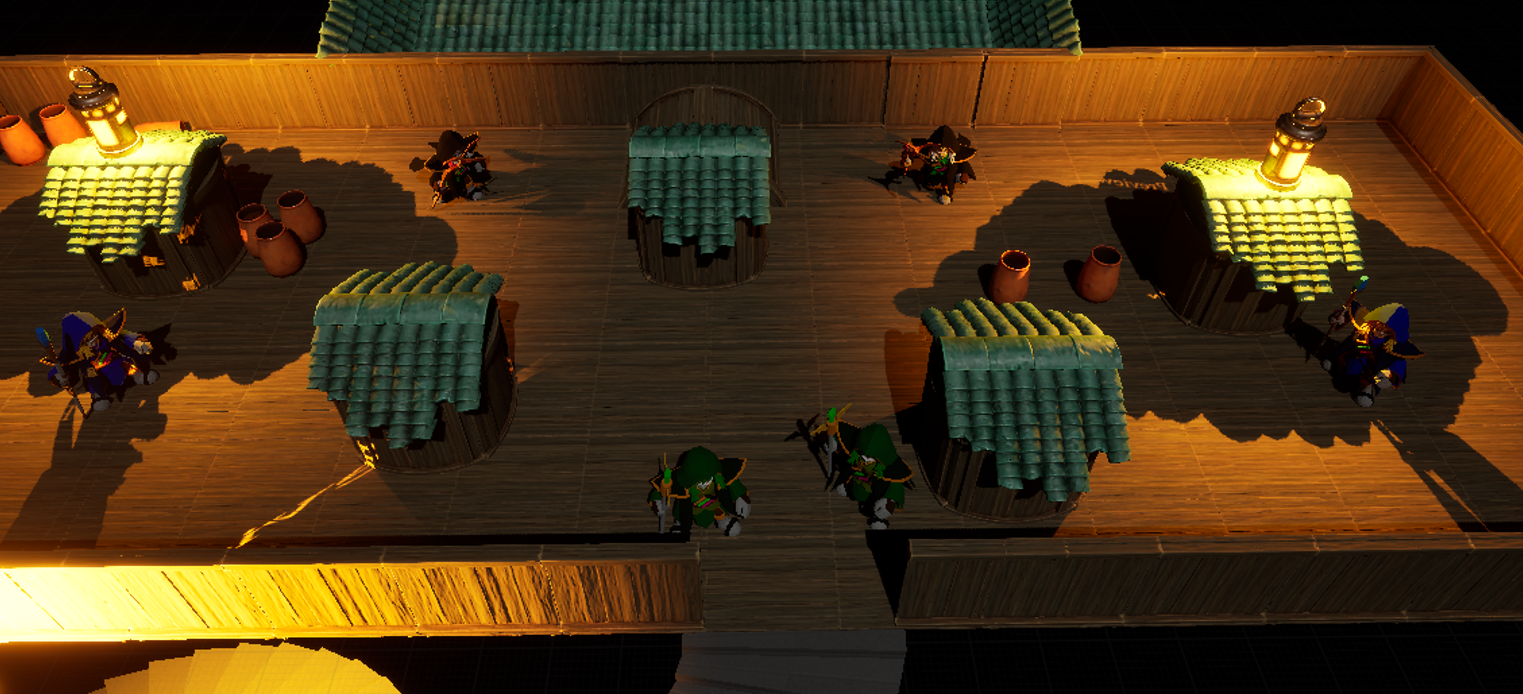
\includegraphics[width=0.5\linewidth]{First Floor (Level 3).png}
    \caption{Erster Bereich in Level 3 mit mehreren Gegnern}
\end{figure}

Im zweiten Stock gibt es eine schmale Plattform. Man darf hier nicht runterfallen, denn unten warten Minigun-Gegner, die einen sofort töten.

\begin{figure}[H]
    \centering
    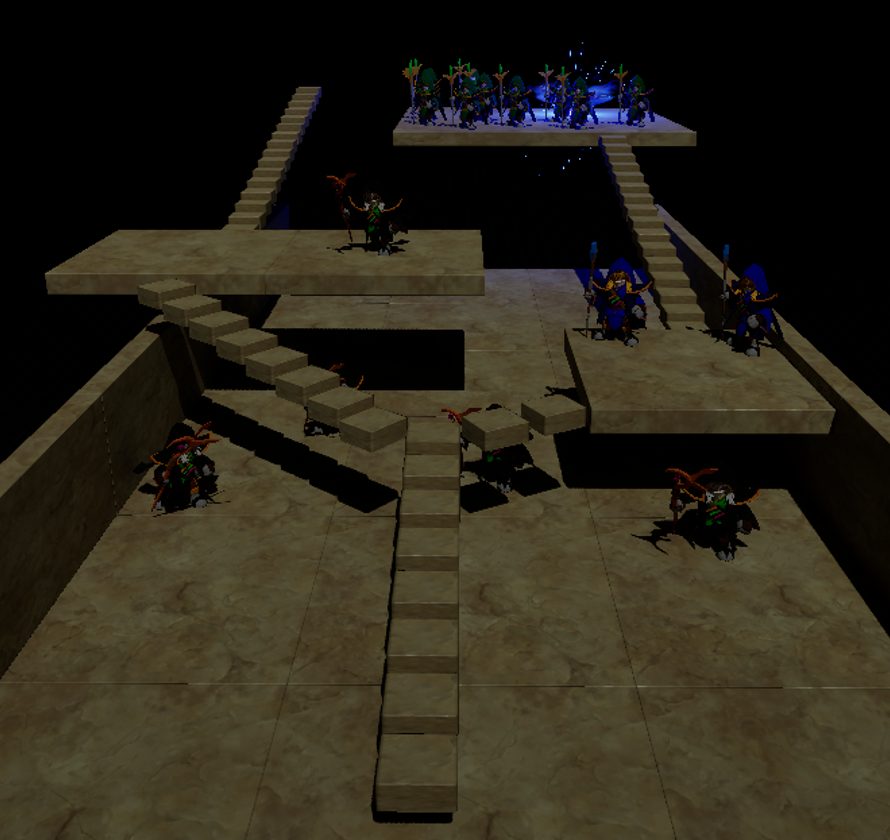
\includegraphics[width=0.5\linewidth]{Second Floor (Level 3).png}
    \caption{Schmale Plattform im zweiten Stock mit tödlichen Minigun-Gegnern unterhalb}
\end{figure}

Am Ende ist das Portal, aber es wird von vielen Gegnern bewacht. Man kann entweder alle aus sicherer Entfernung besiegen oder versuchen, ihren Angriffen auszuweichen und schnell ins Portal zu springen.

\begin{figure}[H]
    \centering
    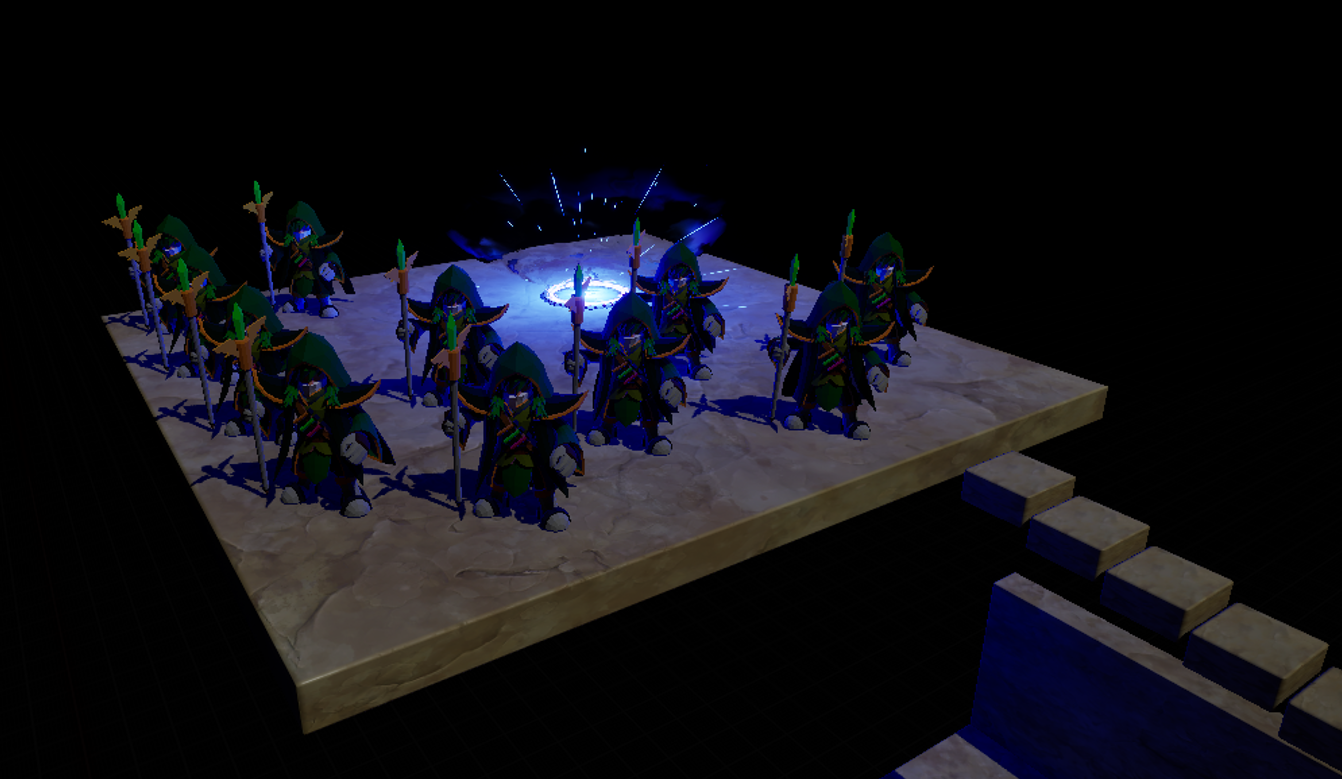
\includegraphics[width=0.5\linewidth]{Enemies near Portal (Level 3).png}
    \caption{Gegner beim Portal im dritten Level}
\end{figure}


\subsection{Level 4}
\label{sub:level4}

\textbf{Level 4} fordert alle bisher erlernten Fähigkeiten des Spielers. Es kombiniert anspruchsvolle Jump’n’Run-Passagen mit gleichzeitigen Kämpfen gegen alle drei Gegnerarten. Die Umgebung ist dynamisch gestaltet, mit Plattformen und Hindernissen, die präzises Timing und strategisches Vorgehen erfordern, um das Portal am Levelende zu erreichen.

In Level 4 wurde insbesondere darauf geachtet ein lebendiges und überzeugendes Leveldesgin zu erschaffen. Somit gibt es keine physikalisch widersprechende Objekte, also z.B. in der Luft schwebend. Dadurch wurde das Gestalten des Levels zwar um einiges komplizierter und aufwendiger, aber das Ergebnise ist ein lebendiges und immersives Level, dass den Spieler überzeugt und gleichzeitg noch mehr spielerische Freiheiten bietet.

Der Spieler durchläuft das Level indem er immer weiter nach oben läuft. Dabei ist zu beachten, dass der Spieler, falls er runterfällt, das Level ohne neuzustarten, weiterspielen kann. Dafür musste extra gesorgt werden, z.B in dem eine Grube und ein Weg zu Beginn des Levels führt. Gelingt es dem Spieler auf die oberste Ebene zu kommen, kann er das Gebäude verlassen und in Richtung Ende springen. Zum Schluss rutscht der Spieler eine tiefe, lange Schräge herrunter. Währenddessen sieht der Spieler von Oben schon das Portal vom Levelende. Das letzte Hindernis ist am Ende der Schräge, sobald der Spieler die Schräge vollkommen runterregutsch ist. Dort findet sich eine mittelgroße Grube. An dieser Grube kann der Spieler entweder ganz einfach rechts bzw. links vorbei laufen oder die angesammelte Geschwindigkeit vom Herunterrutschen nutzen, indem er im richtigen Zeitpunkt springt. Je besser der Spieler das Herunterrutschen zum Boden Aufkommen mit dem Springen zeitlich koordiniert, desto weiter kann er springen und die Grube somit überspringen.
Das Level endet hier in einem dunklen Raum mit ein paar Lichtern, damit es einen visuell flüssigen Übergang zu Level 5 gibt.


\subsection{Level 5}
\label{sub:level5}


\textbf{Level 5} unterscheidet sich durch seine düstere Atmosphäre deutlich von den vorherigen Leveln. Das Level ist als Labyrinth-Adventure gestaltet, in dem der Spieler mithilfe seines Magieschusses den Weg erhellen muss. Mehrere Wege stehen zur Auswahl, doch nur einer führt letztlich zum Portal.

Zu beachten ist, dass der Magieschuss nicht in das „Void“ abgefeuert werden kann. Um die Mechanik korrekt zu nutzen, sollte der Spieler daher in Nähe seiner Spielfigur – idealerweise in Fußnähe – klicken, um zu schießen. 


\section{Steuerung und Eingaben}
\label{sec:steuerungundeingaben}

Die Steuerung wird zu Beginn von Level 1 erläutert und orientiert sich an gängigen Standards, wodurch sie sehr einsteigerfreundlich ist.
Die Bewegung erfolgt über WASD, das Springen mit der Leertaste, und die primäre Aktion – das Abfeuern eines Magieschusses – wird per Linksklick ausgeführt.
Die Schussrichtung richtet sich nach der Position des Mauszeigers, der in die gewünschte Richtung bewegt wird.

Da die Kameraperspektive fest eingestellt ist, bleibt der Mauszeiger dauerhaft eingeblendet und dient als Zielhilfe. Eine freie Kameradrehung, wie sie in vielen Third-Person-Spielen üblich ist, ist hier nicht möglich.

Das Pausenmenü kann jederzeit über die Esc-Taste aufgerufen werden.


\section{Schwierigkeitskurve und Balance}
\label{sec:schwierigkeitskurveundbalance}

Das Spiel beginnt mit einem sehr leichten Schwierigkeitsgrad, sodass der Spieler genügend Zeit hat, sich mit der Steuerung und den Spielmechaniken vertraut zu machen.
In Level 1 und Level 2 lernt man alle Gegnertypen kennen und wird an das grundlegende Movement herangeführt.

In den darauffolgenden Leveln steigt die Schwierigkeit kontinuierlich an: Es treten mehr Gegner auf, und die Jump’n’Run-Passagen werden länger und anspruchsvoller.
Dadurch bleibt das Interesse des Spielers erhalten, da stets eine gewisse Herausforderung geboten wird.

Die Level sind so gestaltet, dass sie nicht zwingend beim ersten Versuch gemeistert werden können, jedoch auch nicht frustrierend lange dauern. Dadurch entsteht ein ausgewogenes Verhältnis zwischen Herausforderung und Spielfluss.


%---
\chapter{Story und Narrative}
\label{cha:stroyundnarrative}

In WTFAI: Where tf am I stürzt die Hauptfigur plötzlich in ein seltsames Rift und findet sich in einer fremden, unheimlichen Welt wieder. Sie hat keine Ahnung, wo sie ist oder wie sie dorthin gekommen ist. Nur eines ist klar: Sie will zurück nach Hause. Um das zu schaffen, muss sie von einem Rift zum nächsten reisen und sich dabei gefährlichen Gegnern, unbekannten Umgebungen und immer neuen Herausforderungen stellen. Die Geschichte wird nicht durch lange Dialoge oder Cutscenes erzählt, sondern durch das, was der Spieler erlebt: die Welt, das Leveldesign und die Atmosphäre. Das Ziel ist klar: nach Hause. Und genau damit beginnt ihre Reise.


%---
\chapter{Grafik und Sound}
\label{cha:grafikundsound}

\section{Visueller Stil und Inspirationsquellen}
\label{sec:visuellerstilundinspirationsquellen}

Anfangs planten wir, dass jedes Gruppenmitglied sein eigenes Level mit einem individuellen Stil gestalten könnte, da das Spielkonzept darauf abzielt, den Spieler in unterschiedliche, unbekannte Welten zu versetzen, in denen er sich orientieren muss. Im Verlauf der Entwicklung entschieden wir uns jedoch für ein einheitliches Fantasy- und realitätsnahes Texturpaket, das kostenlos über Fab erhältlich war: das \textit{Stylized Village Fatpack} von Meshingun Studio. Dieses Paket hat uns visuell überzeugt, da es mit über 450 einzigartigen, modularen Assets, 300 Texturen und mehr als 100 Materialinstanzen eine Vielzahl von Gestaltungsmöglichkeiten bietet. Die enthaltenen Demos zeigten eindrucksvoll, wie vielseitig das Paket ist, was unsere Entscheidung unterstützte. Zudem war es praktisch, da wir unsere Assets auf GitHub hosten und den verfügbaren Speicherplatz begrenzen mussten – das Paket reduzierte den Bedarf an eigenen, speicherintensiven Assets erheblich.

Inspirationen zogen wir aus verschiedenen Spielen, insbesondere aus der Fantasy-Ästhetik und modularen Umgebungen von Titeln wie \textit{Paragon}. Letztendlich haben wir drei helle und zwei dunkle Level. Auf das dunkle Design kamen wir, nachdem wir zufällig die Lichteffekte unseres Magie-Angriffs auf dem Boden reflektiert sahen. Diese Effekte und Lichtreflexionen erhellten den Boden und inspirierten uns zur Gestaltung von Level 5. Zudem wurden wir von verschiedenen Texturpacks und Dungeon-Tutorial-Leveln beeinflusst, deren Designs uns besonders ansprachen.

\section{Farbschema und UI-Design}
\label{sec:farbschemaundui-design}

Das Farbschema und UI-Design wurden bewusst einfach gehalten, um den Fokus des Spielers auf das Spielgeschehen zu lenken. Im Spiel dominieren warme Farben wie Braun, Grün und Gelb in den hellen Leveln, die vom Stylized Village Fatpack inspiriert sind, während die dunklen Level mit dunklen Farbtönen eine mystische Atmosphäre schaffen. Die Anzeige von Hint-Texten während des Gameplays ist um 20 Grad gedreht, damit der Spieler den Text von seiner Ansicht gut lesen kann. Die Textfarbe.  ein Gelbton, wird direkt vom Spieler als Hinweis anerkannt und bindet sich somit harmonisch in die Spielewelt ein. 
Das UI verwendet neutrale Grautöne für Buttons und Menüs, wie im Hauptmenü sichtbar, um sich einfach in die Umgebung einzufügen und Ablenkung zu vermeiden. Die klare, minimalistische Gestaltung mit großen, lesbaren Schriftzügen erleichtert die Navigation und unterstützt die intuitive Bedienung. 


\section{Sounddesign und Musik}
\label{sec:sounddesignundmusik}

Für die musikalische Untermalung von WTFAI wurde gezielt auf passende Stimmungen in den einzelnen Spielbereichen geachtet. Die Hintergrundmusik stammt überwiegend von der Plattform Artlist.io und wurde so ausgewählt, dass sie die Atmosphäre der jeweiligen Level optimal unterstützt – von düster und geheimnisvoll bis hin zu spannungsgeladen und energiegeladen.

Verwendete Musikstücke:

\begin{itemize}
    \item Hauptmenü: Never Die – Noa Lembersky

    \item Level 1–2: Tech No Ledge – Peter Spacey

    \item Level 3: The Battle Ritual – Angel Salazar

    \item Level 4: Keeping Routine – Ran Raiten

    \item Level 5: Heirloom – Jakub Pietras

    \item Death Screen: Folklore (Alternative Version) – Ardie Son
\end{itemize}

Neben der Musik wurden gezielt Soundeffekte eingesetzt, um Spielaktionen klanglich zu verstärken und dem Spieler direktes Feedback zu geben:

Button-Sound: YouTube – \href{https://www.youtube.com/watch?v=h8y0JMVwdmM&ab_channel=SoundLibrary}{Button Sound}

Charakter-Zauber: \href{https://www.youtube.com/watch?v=SJNZDvpGBG8&list=PLpyrFKkVGmcQSYKqGl8Z_dCLQvvtbPMKf&index=13&ab_channel=SoundEffectsSoundCuration}{Character Spell Sound} 

Gegner-Zauber: \href{https://www.youtube.com/watch?v=-f2rxR2GC8s&list=PLpyrFKkVGmcQSYKqGl8Z_dCLQvvtbPMKf&index=9&ab_channel=SoundEffectsSoundCuration}{Enemy Spell Sound}

Zusätzlich stammen zentrale Soundelemente für unseren Hauptcharakter – etwa für Sprung, Schuss, Schadensanzeige und niedrigen Mana-Stand – aus dem Charakterpaket von Fab (UE5 Marketplace).

Insgesamt trägt das Sounddesign maßgeblich dazu bei, die Spielwelt lebendig und stimmungsvoll zu gestalten. Musik und Effekte wurden bewusst eingesetzt, um die emotionale Wirkung und Immersion in den jeweiligen Spielsituationen zu verstärken.


%---
\chapter{KI}
\label{cha:ki}

\section{Feindverhalten und KI-Routinen}
\label{sec:feindverhaltenundki-routinen}

Das Verhalten der feindlichen NPCs sowie ihr Routing sind relativ simpel gehalten.
Sobald der Spieler das Navigation Mesh betritt, bewegt sich der NPC in seine Richtung.
Befindet sich der Spieler beispielsweise auf einer Erhöhung, sucht der NPC nach einer Route innerhalb des Navigation Mesh, die ihn zu dieser Position führt, und folgt dieser.
Findet er keine gültige Route, nähert er sich dem Spieler so weit wie möglich.

Der Angriff des NPCs erfolgt immer in Richtung des Spielers, sobald die Abklingzeit seines Angriffs abgelaufen ist. Die Dauer dieser Abklingzeit variiert je nach Gegnertyp. 

\section{Gegnerarten}
\label{sec:gegnerarten}

Im Spiel gibt es drei Arten von Gegnern. Alle basieren auf derselben EnemyCharacter.cpp-Datei und teilen sich dadurch das gleiche Grundverhalten.

Die drei Gegnertypen unterscheiden sich jedoch in ihrem Design, ihrer Lauf- und Angriffsgeschwindigkeit sowie in den Trefferpunkten.
Die Gegnerarten sind folgende:

  \begin{itemize}
    \item Magier (normal)
        \begin{itemize}
            \item HP: 60
            \item Laufgeschwindigkeit: 200
            \item Angriffsgeschwindigkeit: 3 sec
        \end{itemize}
    \item Schnellschuss-Magier
            \begin{itemize}
            \item HP: 30
            \item Laufgeschwindigkeit: 50
            \item Angriffsgeschwindigkeit: 0,1 sec
        \end{itemize}
    \item Tank-Magier
            \begin{itemize}
            \item HP: 200
            \item Laufgeschwindigkeit: 400
            \item Angriffsgeschwindigkeit: 6 sec
        \end{itemize}
  \end{itemize}

Zum Vergleich: Der Player Character hat eine Laufgeschwindigkeit von 600 und 100 Trefferpunkte. 

%---
\chapter{Technische Umsetzung}
\label{cha:technischeumsetzung}

\section{Game Engine und Tools}
\label{sec:gameengineundtools}

Für die Entwicklung des Spiels wurde die Unreal Engine 5 als Haupt-Engine und primäres Entwicklungswerkzeug verwendet. 
Da wir überwiegend auf Assets aus FAB zurückgegriffen haben, war der Einsatz externer 3D-Tools wie Blender nicht erforderlich. 
Zur Bearbeitung und Optimierung der Soundeffekte kam Audacity zum Einsatz.

\section{Code-Architektur und Struktur}
\label{sec:code-architekturundstruktur}

Die Code-Architektur des Projekts folgt der typischen Struktur der Unreal Engine 5, die auf C++-Klassen und Header-Dateien basiert. 
Zentrale Gameplay-Logik wird in C++-Klassen implementiert, während Header-Dateien die Deklaration von Variablen, Funktionen und Klassen enthalten und so eine klare Trennung zwischen Schnittstelle und Implementierung ermöglichen. 
Das Projekt ist in Module und Unterordner gegliedert (z. B. Characters, Gameplay, UI), um eine saubere und wartbare Struktur zu gewährleisten. 
Die Klassen erben meist von UE5-Basisklassen wie AActor, ACharacter oder UActorComponent, 
was eine einfache Integration in das bestehende Engine-Framework und eine effiziente Nutzung der Engine-Funktionen ermöglicht.

Zudem kamen auf C++-Klassen basierende Blueprints zum Einsatz, um Variablenwerte, Sounds und Meshes zuzuweisen.

%---
\chapter{Entwicklungsprozess}
\label{cha:entwicklungsprozess}

\section{Projektplanung}
\label{sec:projektplanung}

Nach mehreren Besprechungen im Team wurde eine klare Aufgabenteilung festgelegt, um die Entwicklung effizient zu gestalten und die individuellen Stärken der Teammitglieder optimal zu nutzen. 

Die grundlegenden Spielmechaniken wurden gemeinsam definiert:

Das Spiel verfolgt ein einfaches, aber spannendes Ziel. Die Spielerin oder der Spieler muss durch verschiedene Level laufen und dabei Gegner bekämpfen oder ihnen ausweichen, um das Portal zu erreichen. Das Ganze spielt sich in einer Top-Down-Perspektive ab, mit einem primären Angriff auf mittlere Distanz.

Auf dieser Basis wurden die Zuständigkeiten im Team wie folgt verteilt:

\begin{itemize}
    \item Oskar Pokorski war verantwortlich für das Level Design und damit für die Gestaltung der Spielabschnitte und deren Aufbau.
    
    \item Hikmet Gözaydin übernahm die Umsetzung von Menü und Benutzeroberfläche (UI) sowie das gesamte Sounddesign und die musikalische Gestaltung.
    
    \item Niklas Fichtner kümmerte sich um die Implementierung des Hauptcharakters sowie die Entwicklung der Gegnermechanik.
\end{itemize}

Diese Struktur ermöglichte eine klare Aufgabenverteilung und eine koordinierte Umsetzung der Projektziele.


\section{Meilensteine}
\label{sec:meilensteine}

Einige Entwicklungsschritte waren besonders entscheidend für den Fortschritt unseres Projekts, da sie die Grundlage für die weitere Arbeit gelegt haben:

\begin{itemize}
    \item 03.06.2025 – GitHub-Einrichtung & Projektstruktur
    
    Zu Beginn wurde ein gemeinsames GitHub-Repository eingerichtet, inklusive einer strukturierten Projektmappe. Dies war wichtig, um die Zusammenarbeit im Team zu koordinieren, Versionskontrolle zu ermöglichen und einen einheitlichen Arbeitsstand zu sichern. Gleichzeitig wurde das UE5-Projekt aufgesetzt und die grundlegende Ordnerstruktur vorbereitet.
    
    \item 12.06.2025 – Charakter mit Bewegung & Angriff
    
    Die Implementierung der Spielfigur inklusive Movement, Kollisionsverhalten und Angriff auf mittlerer Distanz war ein wichtiger technischer Meilenstein. Erst dadurch konnten Leveltests durchgeführt und das Gameplay erlebbar gemacht werden.
    
    \item 23.06.2025 – Gegner mit Bewegung & Angriff
    
    Mit der Einführung von Gegnern, die sich bewegen und aktiv angreifen, entstand zum ersten Mal echtes Spielgefühl. Diese Mechanik war grundlegend, um das Kampfsystem und die Levelstruktur weiterzuentwickeln.
\end{itemize}

Diese drei Punkte bildeten das Fundament, auf dem alle weiteren Features – wie UI, Leveldesign, Audio oder visuelle Gestaltung – aufgebaut wurden.

Und so sah der Zeitplan für das Projekt aus:

\begin{itemize}
    \item 03.06.2025: Einrichten von Github Repo und Project
    \item 12.06.2025: Charakter mit Movement und Angriff
    \item 12.06.2025: Ui und Menu Design
    \item 12.06.2025: Erste Levels
    \item 23.06.2025: Gegner mit Movement und Angriff
    \item 10.07.2025: Sounddesign & Musik
    \item 12.07.2025: Weitere Level
    \item 16.07.2025: finale Tests und Vorbereitung für die Abgabe
    \item 20.07.2025: Abgabe
\end{itemize}



%---

\chapter{Herausforderungen und Lösungsansätze}
\label{cha:herausforderungenundlösungsansätze}

\section{Einarbeitung}
\label{sec:einarbeitung}

Die Unreal Engine ist eine sehr umfangreiche und komplexe Art von Software. Dadurch kommt man oft zu vielen Schwierigkeiten und Hindernissen. Aufgrund der Bekanntheit und dem Verbreitungsgrad, gibt es jedoch zum Glück sehr viele Resourcen aus denen man lernen kann und seine Probleme lösen kann. Da die Unreal Engine auch stets weiter entwickelt wird, kann man jedoch auch veraltete Resourcen finden, die in der aktuellen Version so nicht funktionieren.

Zur Einarbeitung haben wir verschiedene Resourcen verwendet. Die wichtigsten waren die Unreal Engine Dokumentation auf ihrer Website und unterschiedliche YouTube Anleitungen bzw. komplette Playlists. 
Beim Auftreten von Unklarheiten konnten wir das Problem googlen, in YouTube danach suchen oder uns von einem KI-Modell, wie ChatGPT oder Gemini, helfen lassen. Es war wichtig die grundlegenden Funktionen und das Verhalten der Unreal Engine kennen zu lernen, da man durch bloßes Probieren zwar einiges herausfinden und lernen kann, aber ohne dazugehöriges Wissen, etwas leider einfach nicht versteht.


\section{Technische Probleme}
\label{sec:technischeprobleme}

Ein anfängliches Problem war die Synchronisierung des Projekts über GitHub. Nachdem wir jedoch GitHub LFS sowie eine passende .gitignore für den Upload der relevanten Assets eingerichtet und uns abgestimmt hatten, wer an welcher Map arbeitet, um Merge-Konflikte zu vermeiden, lief die Zusammenarbeit deutlich stabiler.

Wichtig war zudem, nach jedem Pull die C++-Dateien neu zu kompilieren und Unreal anschließend neu zu starten. Nur so konnten neu erstellte C++-Dateien von der Engine und den darauf basierenden Blueprints korrekt erkannt werden.

Ein Problem waren die Systemvorraussetzungen von der Unreal Engine. Sobald die Level ein wenig größer wurden und sich die Anzahl an Materialen und Lichter gehäuft haben, hat sich die Unreal-Editor Performance drastisch verschlechtert. Das betroffene Teammitglied mit einem MacBook Air M1 hat danach einen Cloud-PC von shadow.tech verwendet, um ohne Probleme weiter entwickeln zu können. Diese Lösung hat dann bis zum Projektende sehr gut funktioniert. 

In Level 3 hatten wir kleine Tontöpfe verteilt. Diese haben wir jedoch entfernen müssen. Wenn der Spielercharakter gegen die Töpfe gelaufen ist, hat sich die Bewegungsrichtung des Spielers geändert. Also ist der Charakter durch das Drücken von "W" nicht mehr nach Vorne gelaufen, sondern diagonal rechts nach Vorne zum Beispiel.



\section{Designentscheidungen und Änderungen}
\label{sec:designentscheidungenundänderungen}

Unser Spiel wird von der Top-Down Ansicht gespielt. Auf diese Anforderungen mussten wir beim Leveldesign speziell achten. Dies können wir anhand von Level 4 beispielhaft erklären:

Da Level 4 auf mehreren Ebenen zu spielen sein sollte musste das Level so gestaltet werden, dass dem Spieler nicht von der Decke über ihm die Sicht versperrt wird. Also musste immer ein ausreichend großer Höhenunterschied zwischen den Ebenen beachtet werden. Des Weiteren musste man beachten, wenn man Wände bauen wollte, damit der Spiele nicht außerhalb des Spielbereichs laufen kann, dass diese auch nicht die Sicht des Spielers beeinflussen. Also musste eine Wand hoch genug sein, dass der Spieler nicht darüber springen konnte, aber auch gleichzeitg niedrig genug, dass die Spielansicht nicht beeinflusst wird.

Andere Entscheidungen betrafen die visuelle Integrität des Spiels. Wir haben uns von der ehemaligen Idee mit den mehreren verschieden Designstilen verabschiedet und stattdessen hauptsächlich das Stylized Village Fatpack verwendet.


%---
\chapter{Fazit}
\label{cha:fazit}

\section{Aufgetretene Probleme}
\label{sec:aufgetreteneprobleme}

Die aufgetretenen Probleme waren nahezu ausschließlich technischer Natur und wurden daher bereits im Abschnitt „Technische Probleme“ erläutert.

\section{Erreichte Ziele}
\label{sec:erreichteziele}

Alle im Vorfeld gesetzten Ziele des Projekts konnten erfolgreich erreicht werden. Während der Entwicklung haben wir zahlreiche wertvolle Erfahrungen gesammelt – sowohl auf technischer Ebene, insbesondere im Umgang mit der Unreal Engine 5 und C++, als auch im Bereich der Teamarbeit, Planung und Kommunikation. Die enge Abstimmung im Team und das Lösen technischer Herausforderungen haben maßgeblich zum erfolgreichen Abschluss des Projekts beigetragen.

Das fertige Spiel enthält alle wesentlichen Kernelemente, die ein modernes Spiel auszeichnen. Diese solide Grundlage bietet vielfältige Möglichkeiten für zukünftige Erweiterungen – sei es durch zusätzliche Level, neue Gegnertypen oder erweiterte Gameplay-Mechaniken. Damit bildet das Projekt nicht nur einen erfolgreichen Abschluss unserer Arbeit, sondern auch ein potenzielles Fundament für eine weiterführende Entwicklung.


\section{Weiterentwicklungsmöglichkeiten}
\label{sec:weiterentwicklungsmöglichkeiten}

Obwohl das Spiel in seiner aktuellen Form alle gesetzten Ziele erfüllt, bietet es zahlreiche Ansätze für zukünftige Erweiterungen und Verbesserungen:

\begin{itemize}
    \item Neue Level und Umgebungen: Zusätzliche Level mit variierenden Biomen oder komplexeren Jump’n’Run-Passagen könnten das Spielerlebnis abwechslungsreicher gestalten.
    \item Erweiterte Gegnertypen: Weitere Gegner mit individuellen Angriffsmustern oder KI-Verhalten würden die Kämpfe taktischer machen.
    \item Bosskämpfe: Ein oder mehrere Bossgegner könnten als besondere Herausforderung und Highlight am Ende bestimmter Level dienen.
    \item Verbesserte Spielerprogression: Ein Erfahrungssystem, Upgrades oder freischaltbare Fähigkeiten durch einen Skilltree würden langfristig die Motivation steigern.
\end{itemize}

%---
\chapter{Quellen}
\label{cha:quellen}


\section{Tutorials}
\label{sec:tutorials}

\begin{itemize}
    \item \href{https://dev.epicgames.com/documentation/en-us/unreal-engine/understanding-the-basics-of-unreal-engine}{EpicGames Dokumentation}
    \item \href{https://youtu.be/L9qixi858Ag?feature=shared}{YouTube Video}
    \item \href{https://www.youtube.com/watch?v=4AdGIPV1Yw4}{YouTube Video}
\end{itemize}

\section{Assets}
\label{sec:assets}

\begin{itemize}
    \item \href{https://fab.com/s/e063e89ca643}{Portal}
    \item \href{https://fab.com/s/e780a4984cc7}{Player Character}
    \item \href{https://fab.com/s/66c60dfd1cbf}{Enemy Character}
    \item \href{https://fab.com/s/9d6c2ca3c134}{Materials for Level building}
\end{itemize}

\section{Soundeffects}
\label{sec:soundeffects}

\begin{itemize}
    \item \href{https://www.youtube.com/watch?v=h8y0JMVwdmM&ab_channel=SoundLibrary}{Button sound}
    \item \href{https://www.youtube.com/watch?v=SJNZDvpGBG8&list=PLpyrFKkVGmcQSYKqGl8Z_dCLQvvtbPMKf&index=13&ab_channel=SoundEffectsSoundCuration}{Character spell sound}
    \item \href{https://www.youtube.com/watch?v=-f2rxR2GC8s&list=PLpyrFKkVGmcQSYKqGl8Z_dCLQvvtbPMKf&index=9&ab_channel=SoundEffectsSoundCuration}{Enemy spell sound}
\end{itemize}

%-----------------------------------------------------------------------
\appendix

%---
\printbibliography[heading=bibintoc]



\end{document}
